\chapter{Experiments and Results}
In this section, computer simulation results are presented in a two-dimensional space. The scoring system for formation coordination is validated in Section 4.1. The path planning algorithm is tested via three scenarios in Section 4.2, where the first shows how the team avoids obstacles by spitting and merging, the second shows how the team compress the formation to pass through a narrow area, and the last validates how the team find a solution when encountering a blind alley. The parameters used in our simulation is shown as the below table:


\begin{center}
\captionof{table}{Simulation parameters}
\label{table:combination}
\scalebox{0.9}{ %表格縮放
\begin{tabular}{ll} 
    \Xhline{1.3pt}
    \textbf{parameter} & \textbf{value} \\ 
    \Xhline{1.3pt}
        UAV radius ($r$) & 0.4 $m$\\
        safe distance ($d_{safe}$) & 0.6 $m$\\
        minimum velocity ($v_{min}$) & 0 $m/s$\\
        maximum velocity ($v_{max}$) & 15 $m/s$\\
        maximum acceleration ($a_{max}$) & 0.3 $m/s^{2}$\\
        minimum yaw rate ($\omega_{min}$) & $-40\cdot\frac{\pi}{180}$ $rad/s$\\
        maximum yaw rate ($\omega_{max}$) & $40\cdot\frac{\pi}{180}$ $rad/s$\\
        maximum yaw acceleration ($\omega_{max}$) & $40\cdot\frac{\pi}{180}$ $rad/s$\\

        predicted time ($t_{T}$) &	2 $s$\\
        time tick  &	0.2 $s$\\
    \Xhline{1.3pt}
\end{tabular}}
\end{center}


\section{Validation of The Scoring System}

To fully verify the formation coordination's performance, we use an obstacle-free environment to observe how the UAVs move based on the scoring system. In Figure 4.1, 10 random-positioned UAVs is seen in the bottom-left corner, each of which has a sensing radius $d_{r}$ of 5 meters. After taking off (subgraph a), UAVs instantly detect the neighbors within $d_{r}$ and plan the best trajectories considered the minimum cost in the scoring system. At $t= 5 sec$ (subgraph b), UAVs move closer among neighbors to form compactly. At $t= 10 sec$, final formation is reconfigured (subgraph c). 
Moreover, the final formation differs each time during multiple simulations since our goal is to safely and flexibly show the UAV's behavior. Furthermore, the algorithm shows scalability with the number of UAVs in the above two simulations. Because $N$ does not affect the visual scope, each UAV only has to consider the neighbors as its reference. 


\begin{figure}[htbp]
     \centering
     \begin{subfigure}[b]{0.3\textwidth}
         \centering
         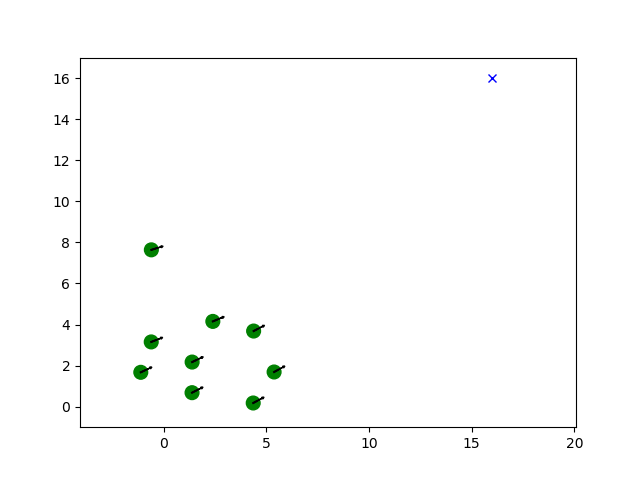
\includegraphics[width=\textwidth]{figures/reconfigure_1.png}
         \caption{random positioned UAV}
         \label{before merging}
     \end{subfigure}
     \hfill
     \begin{subfigure}[b]{0.3\textwidth}
         \centering
         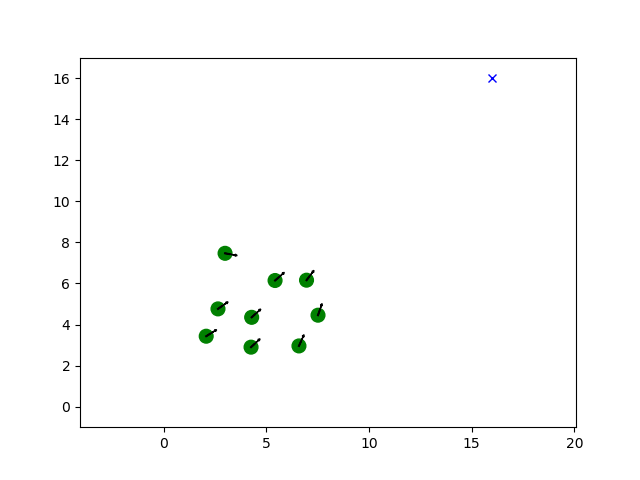
\includegraphics[width=\textwidth]{figures/reconfigure_2.png}
         \caption{formation coordination}
         \label{ew}
     \end{subfigure}
     \hfill
     \begin{subfigure}[b]{0.3\textwidth}
         \centering
         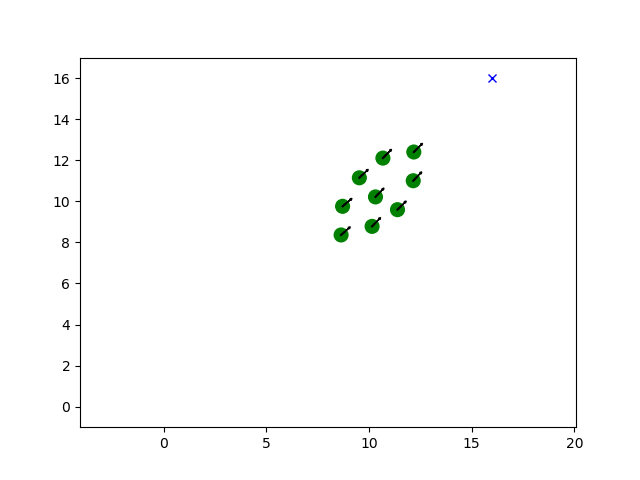
\includegraphics[width=\textwidth]{figures/reconfigure_3.png}
         \caption{final formation}
         \label{qw}
     \end{subfigure}
        \caption{Reconfiguring a compact formation}
        \label{fig}
\end{figure}


In the second simulation (Figure 4.2), we separate 10 UAVs into two groups and observe the behavior between them while flying toward the same goal point. At the beginning (subgraph a), two groups of 5 UAVs are positioned separately. At $t=5$, several UAV's sensors in both groups detect the position of the other group, which increase the number of neighbors. Therefore, the two groups merge into a team and form a new formation at $t=15$. 

\begin{figure}[htbp] 
     \centering
     \begin{subfigure}[b]{0.3\textwidth}
         \centering
         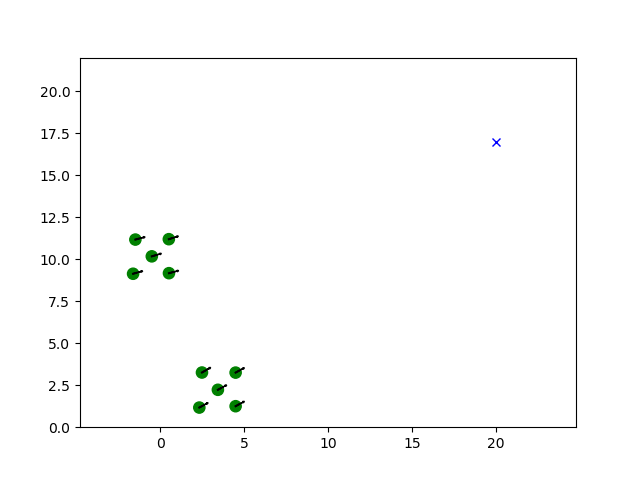
\includegraphics[width=\textwidth]{figures/merge_1.png}
         \caption{before merging}
         \label{fig:y equals x}
     \end{subfigure}
     \hfill
     \begin{subfigure}[b]{0.3\textwidth}
         \centering
         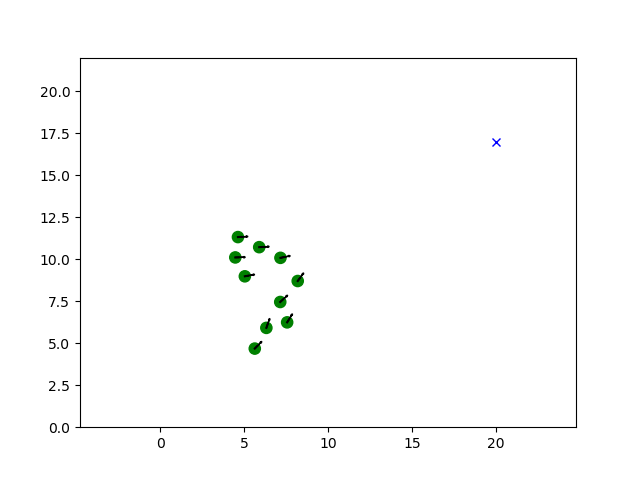
\includegraphics[width=\textwidth]{figures/merge_2.png}
         \caption{formation coordination}
         \label{fig:three sin x}
     \end{subfigure}
     \hfill
     \begin{subfigure}[b]{0.3\textwidth}
         \centering
         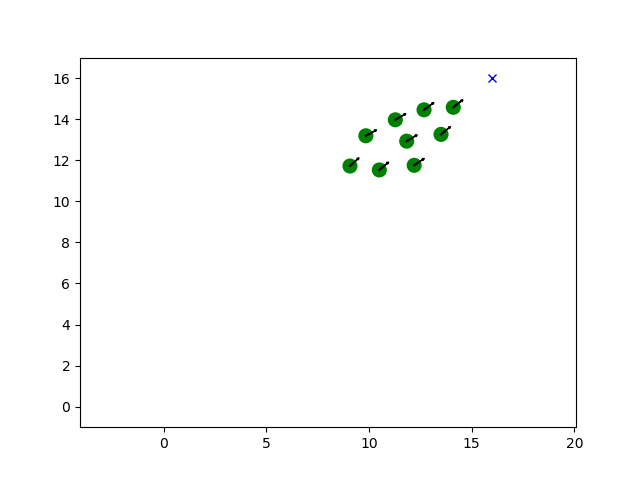
\includegraphics[width=\textwidth]{figures/merge_3.png}
         \caption{after merging}
         \label{fig:five over x}
     \end{subfigure}
        \caption{Formation merging of two groups}
        \label{fig:three graphs}
\end{figure}

\section{Validation of Comprehensive Performance}
\subsection{Obstacle avoidance}
We set up an environment with multiple obstacles dispersed randomly with a radius from 0.2 (m) to 1.5 (m) in the flight space. The goal point is set at (24, 24), and a formation flight for a team is considered to start from the left-down corner. The team consists of six UAVs, which the initial positions are set to (1, 5), (3, 5), (5, 5), (3, 3), (5, 3), (5, 1) respectively, and their predefined trajectories are straight lines toward the goal point.

The result is shown in Figure 4.2, where colored-dashed lines denote the trajectories corresponding to each UAV. The group separates in the beginning to avoid the small obstacle placed in (9, 9), and they then merge into a group after passing it. Before reaching the goal point, the split again to dodge the bigger obstacle successfully.

\begin{figure}[H]
    \centering
    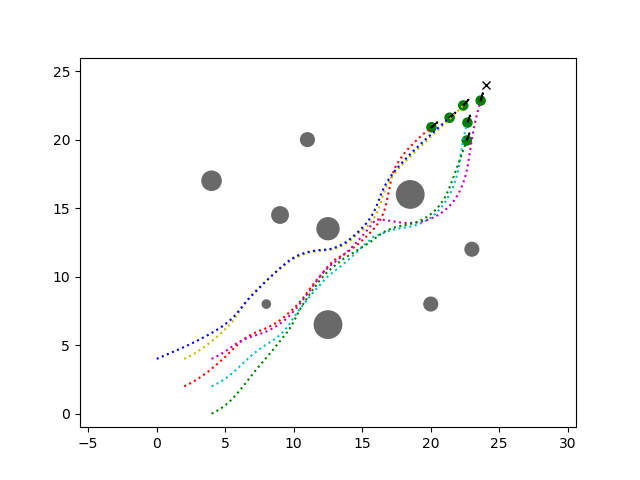
\includegraphics[scale=0.7]{figures/exp1-3.png}
    \caption{Overall trajectories for obstacles avoidance}
    \label{fig:fig_label}
\end{figure}

\subsection{Passing through a narrow area}
To test the capability of formation compression, we set up a narrow area for the UAV team to pass through. In the simulation, UAVs should switch the state $flying$ to state $waiting$ before passing through the narrow trail. The result is shown in Figure 4.3, where a team of 8 UAVs start from the left and the goal point is set on the right. In Figure 4.4, we use the color for UAVs to identify the states while passing through the trail, where the green UAVs represent the ones in a $flying$ state and the black ones are for the $waiting$ state. It is evident that both sides of the UAV predict the inter-vehicle may occur before entering, and therefore they wait for the former teammates.

\begin{figure}[H]
    \centering
    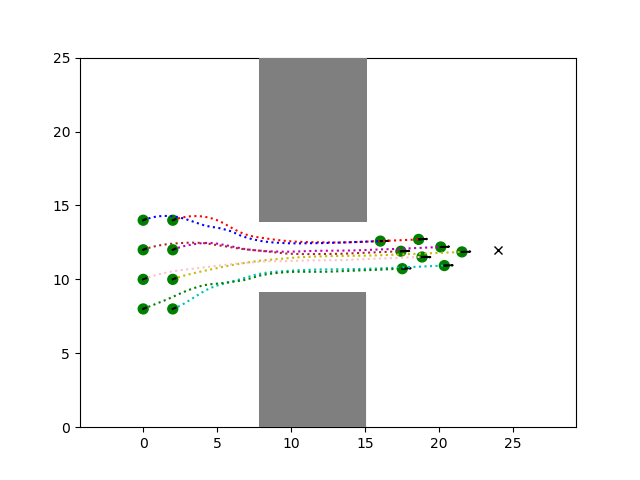
\includegraphics[scale=1]{figures/trail_overall.png}
    \caption{Overall trajectories in a narrow trail}
    \label{fig:fig_label}
\end{figure}
\begin{figure}[H]
    \centering
    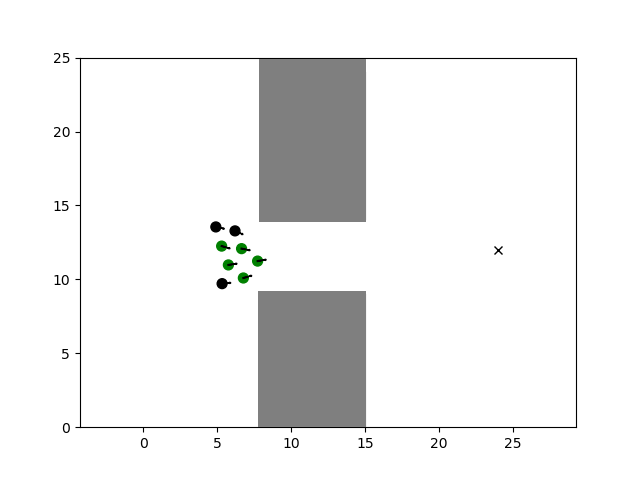
\includegraphics[scale=1]{figures/trail_enter.png}
    \caption{waiting state validation}
    \label{fig:fig_label}
\end{figure}

\subsection{Maze-like environment}
More complex obstacles are placed on testing comprehensive functionality. Due to the limited sensor, UAVs cannot predict the obstacles that might block the direction in advance. Our algorithm requires neither leader nor fixed formation so that the team can easily fly in the opposite direction, and find another solution. 

Figure 4.5 shows that the 6 UAVs are blocked in the beginning after they move for a short distance. Nevertheless, the pioneers invoke the state $searching$ when there is no available path. On the other hand, the UAVs behind switch the state $flying$ to $waiting$ and wait for their teammates. To prevent deadlock, We preset the constant $clock$ to 2 seconds. That is, every UAV will start to navigate new paths after the time-out. Finally, it can be seen that the team successfully find another route and fly toward the goal point.

\begin{figure}[H]
    \centering
    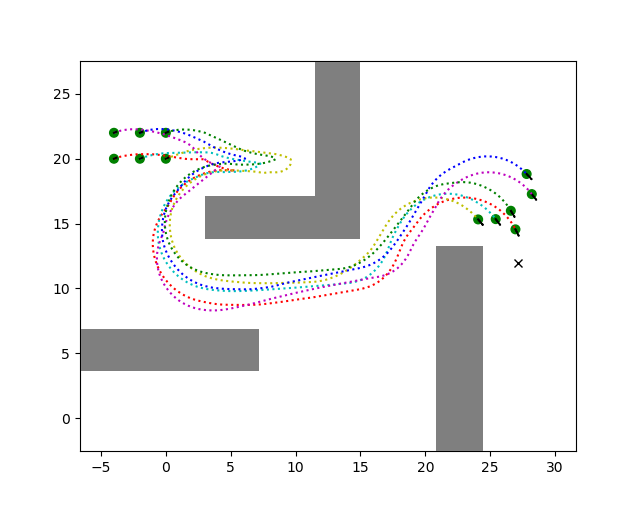
\includegraphics[scale=1]{figures/comprehensive_simulation_2.png}
    \caption{\label{tab:table-name} UAVs fly in a maze-like environment}
    \label{fig:fig_label}
\end{figure}
